\documentclass[tikz,border=2pt]{standalone}
\usepackage{amsmath}
\usepackage{pgfplots}
\pgfplotsset{compat=1.18}
\usetikzlibrary{arrows.meta}
\begin{document}
% Strong duality on Example 5.1: primal feasible values fill [0,36], dual feasible values fill [36,infinity);
% they meet at Z*=W*=36, attained by x*=(2,6) and y*=(0,3/2,1). The pair x=(4,3), y=(0,2,1) has 27<42.
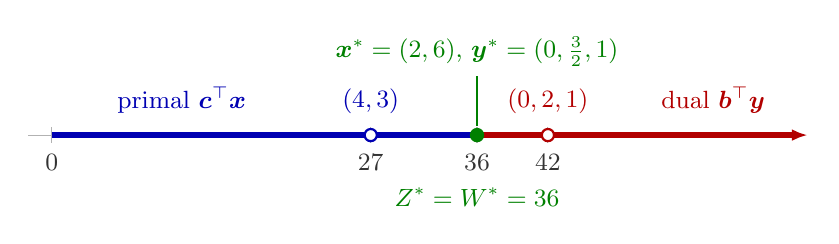
\begin{tikzpicture}[font=\small, >={Latex[length=2mm]}, x=0.15cm, y=1cm]
  % axis
  \draw[gray!60] (-2,0) -- (0,0);
  \foreach \v in {0,27,36,42} {
    \draw[gray!60] (\v,0.1) -- (\v,-0.1);
    \node[gray!40!black, anchor=north] at (\v,-0.12) {$\v$};
  }
  % ranges of values
  \draw[blue!70!black, line width=2.2pt] (0,0) -- (36,0);
  \draw[red!70!black, line width=2.2pt, ->] (36,0) -- (64,0);
  \node[blue!70!black, anchor=south] at (11,0.15) {primal $\boldsymbol{c}^{\top}\boldsymbol{x}$};
  \node[red!70!black, anchor=south] at (56,0.15) {dual $\boldsymbol{b}^{\top}\boldsymbol{y}$};
  % a non-optimal feasible pair
  \filldraw[blue!70!black, fill=white, thick] (27,0) circle (2.2pt);
  \node[blue!70!black, anchor=south] at (27,0.15) {$(4,3)$};
  \filldraw[red!70!black, fill=white, thick] (42,0) circle (2.2pt);
  \node[red!70!black, anchor=south] at (42,0.15) {$(0,2,1)$};
  % the common optimum
  \fill[green!50!black] (36,0) circle (2.6pt);
  \draw[green!50!black] (36,0.12) -- (36,0.75);
  \node[green!50!black, anchor=south] at (36,0.75) {$\boldsymbol{x}^{\ast}=(2,6)$,\ $\boldsymbol{y}^{\ast}=(0,\tfrac{3}{2},1)$};
  \node[green!50!black, anchor=north] at (36,-0.55) {$Z^{\ast}=W^{\ast}=36$};
\end{tikzpicture}
\end{document}
